\documentclass[10pt,letterpaper]{memoir}
% memoir commands to define the text block geometry
\setulmarginsandblock{0.75in}{*}{*}
\setlrmarginsandblock{0.75in}{*}{*}

\usepackage{xparse}
\usepackage{blindtext}
\usepackage{enumitem}
\usepackage{graphicx}

\usepackage{amsmath,mathtools,amssymb}
% See https://texblog.net/latex-archive/maths/amsmath-matrix/ 
% for an explanation of this extention of the amsmath matrix commands.
% It's a way to enable "augmented matrices" using a new optional argument:
%
% \begin{pmatrix}[cc|c]
%     1 & 2 & 3\\
%     4 & 5 & 9
%   \end{pmatrix}
%
\makeatletter
\renewcommand*\env@matrix[1][*\c@MaxMatrixCols c]{%
  \hskip -\arraycolsep
  \let\@ifnextchar\new@ifnextchar
  \array{#1}}
\makeatother

\usepackage{bm} % bold math package

\usepackage{booktabs}
\usepackage{multirow}
\usepackage{hyperref}
\usepackage{systeme}

\usepackage{tcolorbox}
    \tcbuselibrary{skins}
    \tcbuselibrary{raster}
    \tcbuselibrary{skins}
\usepackage{tikz}
    \usetikzlibrary{arrows.meta}
\usepackage{tkz-base}
\usepackage{tkz-fct}    
\usepackage{pgfplots}
    \pgfplotsset{compat=newest}

% for inserting blanks that the students fill in
\usepackage{dashundergaps} % for \gap
\dashundergapssetup{
    teacher-mode=false, % set to true to show answers 
    gap-format=underline,
    teacher-gap-format=underline,
    gap-font={\ECFAugie\MTversion{augie}\color{black}},
    gap-numbers=false,
    gap-widen=true,
    gap-extend-percent=100, % note: making this too big might create errors
    gap-number-format=\,\textsuperscript{\normalfont(\thegapnumber)},
}

\usepackage{emerald}
\usepackage[subdued]{mathastext}% no italic for Augie anyhow
    \MTDeclareVersion[n]{lmvtt}{T1}{lmvtt}{m}{n}
    \MTfamily{augie}
    \Mathastext[augie]

\newcommand{\myHeadFootStyle}{\footnotesize\sffamily}
\copypagestyle{myPagestyle}{empty}
%
% FIXME
% The following header definitions do NOT work right in all cases.
% I have found that the chapter title sometimes gets picked up from
% a chapter that begins on the NEXT PAGE. Not sure what's going on.
% So I abandoned embedding the info in the header and instead updated
% \myLesson to print it out, and that seems to work find.
%
% \makeoddhead{myPagestyle}
%     {\,}
%     {\,}
%     {\myHeadFootStyle\chaptername\,\thechapter\,\,\myCurrentChapterTitle}
% \makeevenhead{myPagestyle} 
%     {\,}
%     {\,}
%     {\myHeadFootStyle\chaptername\,\thechapter\,\,\myCurrentChapterTitle}
\makeoddfoot{myPagestyle}
    {\myHeadFootStyle\myCurrentBookTitle}
    {\myHeadFootStyle\thepage}
    {\myHeadFootStyle\thechapter.\themyLessonCounter\,\,\myCurrentLessonTitle}
\makeevenfoot{myPagestyle}
    {\myHeadFootStyle\thechapter.\themyLessonCounter\,\,\myCurrentLessonTitle}
    {\myHeadFootStyle\thepage}
    {\myHeadFootStyle\myCurrentBookTitle}


\setlength{\parindent}{0em}
\setlength{\parskip}{0.75em}

\begin{document}
\pagestyle{plain}
\checkandfixthelayout
% \raggedbottom

\newcommand{\myEmph}{\bfseries\itshape}
\newcommand{\myClassName}{{\tagged{pre-AP}{pre-AP }}Algebra 2}

% So I can save/restore \fboxsep
\newlength{\mySavedFboxsep}
\newcommand{\mySaveFboxsep}{\setlength{\mySavedFboxsep}{\fboxsep}}
\newcommand{\mySaveAndSetFboxsep}[1]{
    \setlength{\mySavedFboxsep}{\fboxsep}
    \setlength{\fboxsep}{#1}
}
\newcommand{\myRestoreFboxsep}{\setlength{\fboxsep}{\mySavedFboxsep}}

% A centered tcolorbox
%
% #1 - options to pass to tcolorbox
%
\NewDocumentEnvironment{myCenteredBox}{m}{%
    \begin{center}
    \begin{tcolorbox}[#1]
}{
    \end{tcolorbox}
    \end{center}
}


% A centered system of equations
%
\NewDocumentCommand{\myCenteredSysteme}{m}{%
    \begin{center}\systeme{#1}\end{center}
}

%
% This specialized command is my way of typesetting a table for
% students to use when solving systems of equations using matrices.
%
% - I make it really wide, because I need horizontal space. The increase in margin width 
%   is adjustable, but frankly, there are a lot of hard-coded dimensions in the table, so
%   I'm not positive that generality works well.
%
% - I put the content in a tikz picture with an OPAQUE background, since I 
%   plan to overlay this on top of Examples, which have dotted boxes around 
%   them at the "normal" margins.
%
% - The table uses the multirow package so that I can have the "Solution" box span two cells.
%
\NewDocumentCommand{\myWideMatrixTable}{O{-0.7in}}{
    \begin{adjustwidth}{#1}{#1}
        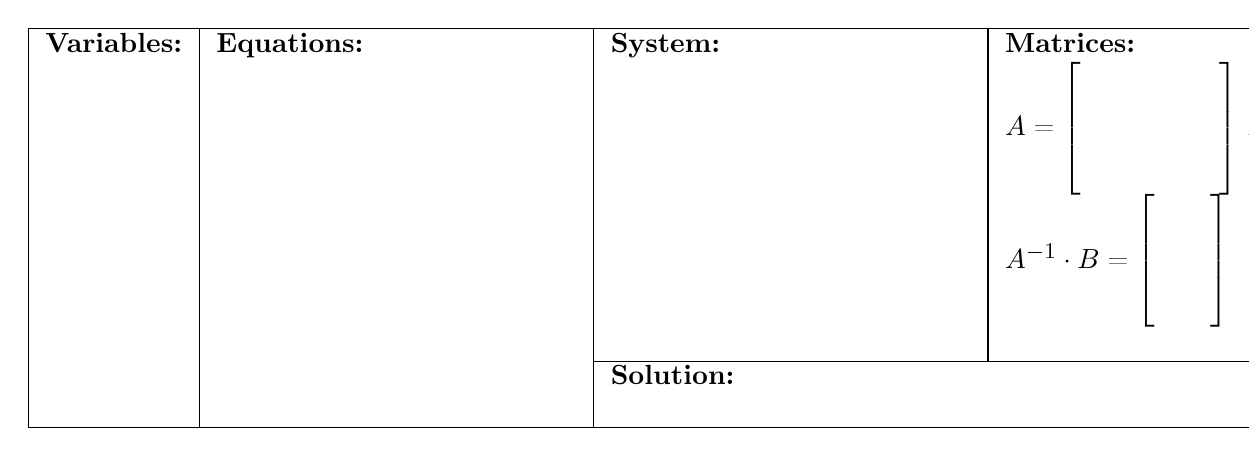
\begin{tikzpicture}
            \node
            [
                text width=1.25\textwidth, %I dinked with the multiplier to get balanced margins
                fill=white!30, 
                fill opacity=1,
                text opacity=1,
                inner sep=0pt,
            ]
            {%
                \begin{tabular}{|l|m{1.8in}|m{1.8in}|m{2.1in}|}
                    \hline
                    {\bfseries\scshape Variables:} & {\bfseries\scshape Equations:} & {\bfseries\scshape System:} & {\bfseries\scshape Matrices:} \\
                    % & & & \\
                    & & & 
                    \(
                        A = 
                        \begin{bmatrix}
                            \phantom{99} & \phantom{99} & \phantom{99} \\
                            \phantom{99} & \phantom{99} & \phantom{99} \\
                            \phantom{99} & \phantom{99} & \phantom{99} \\
                            \phantom{99} & \phantom{99} & \phantom{99} \\
                        \end{bmatrix}
                    \)
                    \(
                        B = 
                        \begin{bmatrix}
                            \phantom{999}\\
                            \phantom{999}\\
                            \phantom{999}\\
                            \phantom{999}\\
                    \end{bmatrix}
                    \)
                    \\
                    & & &
                    \(
                        A^{-1}\cdot B = 
                        \begin{bmatrix}
                            \phantom{9999}\\
                            \phantom{999}\\
                            \phantom{999}\\
                            \phantom{999}\\
                    \end{bmatrix}
                    \)
                    \\
                    & & & \\ \cline{3-4}
                    & & 
                    \multicolumn{2}{l|}{\bfseries\scshape Solution:}
                    \\ 
                    & & 
                    \multicolumn{2}{l|}{\,}
                    \\ 
                    \hline
                \end{tabular}
            };
        \end{tikzpicture}
    \end{adjustwidth}
}


{\small Pre-AP Algebra 2}\hfill Name: \rule{2in}{0.15mm}

{\Large PAP HW 4.4 Matrix Applications}\hfill Period: \rule{0.5in}{0.15mm}

{\itshape
For the following problems, translate the problem into a system of linear equations,
and solve those equations using the Desmos matrix calculator at {\ttfamily desmos.com/matrix}.
\vspace{1.5em}
}




{\bfseries\large 1)} 
You find a jar of dimes and quarters.
There is a total of 70 coins in the jar.
When you take them to the bank (to the coin counting machine),
you find that they added up to \$13.00.
How many dimes and how many quarters were in the jar?

\myWideMatrixTable[-0.1in]
\vspace{0.5in}
\hfill{\itshape (Ans: 30 dimes, 40 quarters)}
\vspace{2em}




{\bfseries\large 2)} 
You find another jar of 120 pennies, nickles and dimes.
You just happen to know that there are 10 fewer nickles than dimes
(or equivalently, there are ten more dimes than nickles).
When you take them to the bank (to the coin counting machine),
you find that they added up to \$6.00.
How many pennies, nickles, and dimes were in the jar?

\myWideMatrixTable[-0.1in]

\vspace{0.5in}
\hfill{\itshape (Ans: 50 pennies, 30 nickles, 40 dimes)}
\vspace{2em}



\newpage
{\bfseries\large 3)} 
Jazmin's Restaurant ordered 200 flowers for the holidays.
They ordered carnations, roses and daisies.
They ordered 20 fewer roses than daisies
(or equivalently, 20 more daisies than roses).
The carnations cost \$1.50 each.
The roses cost \$5.75 each.
The daisies cost \$2.60 each.
The total cost of the order was \%589.50.
How many of each kind of flower did they order?

\myWideMatrixTable[-0.1in]

\vspace{0.5in}
\hfill{\itshape (Ans: 80 carnations, 50 roses, 70 daisies)}
\vspace{2em}




{\bfseries\large 4)} 
Arly's Game Arcade uses three different kinds of tokens for their game machines.
There are gold tokens.
There are silver tokens.
There are bronze tokens.
For \$20.00, you can buy any of the following mixes of tokens:
\begin{itemize}[itemsep=0in]
    \item 14 gold, 20 silver, 24 bronze
    \item 20 gold, 15 silver, 19 bronze
    \item 30 gold, 5 silver, 13 bronze.
\end{itemize}
How much does each kind of token cost?

\myWideMatrixTable[-0.1in]

\vspace{0.5in}
\hfill{\itshape (Ans: gold: \$0.50, silver: \$0.35, bronze: \$0.25)}
\vspace{2em}




\newpage
{\bfseries\large 5)} 
Last weekend, the Nostream Movie Theater sold a total of 8500 movie tickets.
They earned \$64,600.00.
Tickets are sold in one of three ways:
\begin{itemize}
    \item A matinee (early show) ticket costs \$5.00.
    \item A student all-day ticket costs \$6.00.
    \item Regular tickets cost \$8.50.
\end{itemize}
They sold twice as many student tickets as matinee tickets.
How many of teach kind of ticket did they sell?

\myWideMatrixTable[-0.1in]

\vspace{0.5in}
\hfill{\itshape (Ans: 900 matinee, 1800 student, 5800 regular)}
\vspace{2em}




{\bfseries\large 6)} 
Rudy's Ripoff Tienda sells hats, T-shirts, and jackets. 
You know the following three facts:
\begin{itemize}[itemsep=0in]
    \item Three hats, two T-shirts, and one jacket cost \$140.00.
    \item Two hats, two T-shirts, and two jackets cost \$170.00.
    \item One hat, three T-shirts, and two jackets cost \$180.00.
\end{itemize}
What is the cost of each of these three items?

\myWideMatrixTable[-0.1in]

\vspace{0.5in}
\hfill{\itshape (Ans: hat: \$15.00, T-shirt: \$25.00, jacket: \$45.00)}
\vspace{2em}



\newpage
{\bfseries\large 7)} 
Guadalupe, Jennifer, and Karla work at Notear Jeans Company.
One day, the three of them sold a combined \$1480.00 worth of jeans.
Guadalupe sold \$120.00 more than Jennifer.
Jennifer and Karla together sold \$280.00 more than Guadalupe.
How much did each of them sell?

\myWideMatrixTable[-0.1in]

\vspace{0.5in}
\hfill{\itshape (Ans: Guadalupe: \$600.00, Jennifer: \$480.00, Karla: \$400.00)}
\vspace{2em}




{\bfseries\large 8)} 
Guadalupe, Jonathan, and Kevin work at Topnotch Boot Company.
One day, the three of them sold a combined \$1550.00 worth of boots.
Guadalupe sold \$150.00 more than Jonathan.
Kevin sold \$250.00 less than Guadalupe.
How much did each of them sell?

\myWideMatrixTable[-0.1in]

\vspace{0.5in}
\hfill{\itshape (Ans: Guadalupe: \$650.00, Jonathan: \$500.00, Karla: \$400.00)}
\vspace{2em}


\end{document}